\documentclass[11pt]{beamer}
\usetheme{CambridgeUS}
\usepackage[utf8]{inputenc}
\usepackage[spanish]{babel}
\usepackage{amsmath}
\usepackage{amsfonts}
\usepackage{amssymb}
\usepackage{graphicx}
\usepackage{ragged2e}
\setbeamertemplate{navigation symbols}{} 
\author[Kevin García - Alejandro Vargas]{Kevin García 1533173 \newline Alejandro Vargas 1525953}
\title[Anteproyecto]{Diseño y validación de muestreo de cítricos para detección de enfermedades en viveros del Valle del Cauca}


\newcommand\Wider[2][1em]{%
\makebox[\linewidth][c]{%
  \begin{minipage}{\dimexpr\textwidth+#1\relax}
  \raggedright#2
  \end{minipage}%
  }%
}


%\setbeamercovered{transparent} 
%\setbeamertemplate{navigation symbols}{} 
%\logo{} 
%\institute{} 
%\date{} 
%\subject{} 
\begin{document}
\justify
\begin{frame}
\titlepage
\end{frame}

%\begin{frame}
%\tableofcontents
%\end{frame}

\begin{frame}
\frametitle{Contenido}
\begin{itemize}
\item Información del proyecto
\item Problema Contextual
\item Problema Estadístico
\item Objetivos
\item Variable de interés
\item Antecedentes
\begin{itemize}
\item Antecedentes Contextuales
\item Antecedentes Estadísticos
\end{itemize}
\item Marco Teórico
\end{itemize}
\end{frame}

\begin{frame}
\frametitle{Información del proyecto}
\begin{itemize}
\item Entidad encargada: AGROSAVIA (Corpoica)
~\\La Corporación Colombiana de Investigación Agropecuaria, Corpoica, es una entidad pública descentralizada de participación mixta sin ánimo de lucro, de carácter científico y técnico, cuyo objeto es desarrollar y ejecutar actividades de Investigación, Tecnología y transferir procesos de Innovación tecnológica al sector agropecuario.

~\\
\item Personal a cargo:
\begin{itemize}
\item[-]Nubia Murcia Riaño (Investigador Ph.D.)
\item[-]Mauricio Fernando Martínez (Investigador Máster)
\item[-]Elizabeth Narvaez Toro (Líder de Seguimiento y Evaluación)
\end{itemize}
\end{itemize}
\end{frame}


\begin{frame}
\frametitle{Problema Contextual}
~\\Existen diversas enfermedades en los cítricos transmitidas principalmente por injertación, vectores (organismos o insectos), y uso de herramienta, las cuales son muy dañinas para este cultivo, entre ellas, el virus de la tristeza, HLB, Leprosis y Exocortis. Estas debilitan el árbol, generando producciones escasas, y en casos avanzados puede llegar a matar el árbol. El inconveniente es que estas enfermedades son asintomáticas en edades tempranas de la planta, es decir, no podemos diferenciar a simple vista una planta infectada con una no infectada. Al sembrar una planta con alguna de estas infecciones desde el comienzo, se perderá mucho dinero invirtiendo en su mantenimiento, por lo cuál se necesita asegurar o garantizar que las plantas que van a ser sembradas y entregadas estén limpias de estas enfermedades, logrando de esta manera la producción de material certificado.
\end{frame}

\begin{frame}
\frametitle{Problema Estadístico}
~\\Partiendo del problema contextual, surgen las siguientes preguntas
\begin{itemize}
\item ¿Es posible diseñar un plan de muestreo adecuado y asequible que permita la detección temprana de estas enfermedades en los cítricos?
\item ¿Es posible estimar la cantidad de plantas infectadas en los lotes a partir del plan de muestreo diseñado?
\end{itemize}
\end{frame}

\begin{frame}
\frametitle{Objetivos propuestos}
\begin{itemize}
\item Objetivo General
~\\Diseñar y validar un plan de muestreo para aceptación y rechazo de lotes de cítricos en viveros del Valle del Cauca que permita estimar la cantidad de plantas infectadas con el virus de la tristeza en el lote.
\item Objetivos Específicos
\begin{itemize}
\item[-]Proponer y diseñar diferentes tipos de muestreo tipo aceptación/rechazo para lotes de cítricos en viveros del Valle del Cauca.
\item[-]Validar los diseños muéstrales por medio de simulación teniendo en cuenta confianza y costo del muestreo.
\item[-]Estimar la cantidad de plantas infectadas con el virus de la tristeza.
\end{itemize}
\end{itemize}
\end{frame}

\begin{frame}
\frametitle{Variable de interés}
~\\Nuestra variable de interés se puede definir de la siguiente manera:
$$X= \left\{\begin{array}{cc}
             1 &   si \; la \; planta \; esta \; infectada \\
             \\ 0 &  si \; la \; planta \; no \; esta \; infectada \\
             \end{array}
   \right.$$
\end{frame}


\begin{frame}
\frametitle{Variable de interés}
~\\Para llegar a la variable de interés definida anteriormente, se lleva a cabo una prueba de laboratorio en la cuál se pueden medir hasta 45 muestras de tejido de plantas, donde se obtiene al final una coloración en el recipiente, a esta coloración se le hace una lectura visual o colorimétrica, usualmente se utiliza más la medida colorimétrica por ser mas objetiva, esta se obtiene con un valor de absorbancia, que corresponde en pocas palabras a una cuantificación de la percepción del color. Se encuentra de la siguiente manera:
\[ A_\lambda=-log_{10} \left( \frac{I}{I_0}\right) \]
~\\Donde:
~\\I es la intensidad de la luz con una longitud de onda específica $\lambda$ tras haber atravesado una muestra (intensidad de la luz transmitida).
~\\$I_0$  es la intensidad de la luz antes de entrar a la muestra (intensidad de la luz incidente).
\end{frame}

\begin{frame}
\frametitle{Antecedentes}
\begin{itemize}
\item Antecedentes Contextuales
\begin{itemize}
\item[1.]Vidal, E. (2010). Epidemiología de Plum pox virus y citrus tristeza virus en bloques de plantas de vivero. Métodos de control (Tesis doctoral). Universitat Politécnica de Valencia, Valencia, España.
\item[2.]Pérez,A. , Mora, B. , León, M. , García, J. \& Abad, P. (2012). Enfermedades causadas por Phytophthora en viveros de plantas ornamentales (Artículo). Universitat Politécnica de Valencia, Valencia, España. Bol. San. Veg. Plagas, 38: 143-156.
\item[3.]Parke, J. L., Knaus, B. J., Fieland, V. J., Lewis, C., and Grünwald, N. J.
2014. Phytophthora community structure analyses in Oregon nurseries
inform systems approaches to disease management. Phytopathology
104:1052-1062.
\end{itemize}
\end{itemize}
\end{frame}

\begin{frame}
\frametitle{Antecedentes}
\begin{itemize}
\item Antecedentes Contextuales
\begin{itemize}
\item[4.]Caribbean food crops society. (2008).El Virus de la Tristeza de los Citricos (CTV) en Plantaciones Comerciales y Viveros
de la Repûblica Dominicana.(Plenary Session and Oral Presentations). University of Florida.
\item[5.]Melgara,(2018).Ocurrencia de Huanglongbing (Candidatus Liberibacter asiaticus) y su vector [Diaphorina citri Kuwayama (Hemiptera: Liviidae)] en viveros de cítricos de Masaya.(Trabajo de Graduación, MAESTRÍA EN SANIDAD VEGETAL).UNIVERSIDAD NACIONAL AGRARIA
FACULTAD DE AGRONOMIA
\end{itemize}
\end{itemize}
\end{frame}

\begin{frame}
\frametitle{Antecedentes}
\begin{itemize}
\item Antecedentes Estadísticos
\begin{itemize}
\item[1.]Abad Corpa, E. , Leal Llopis, J. , Paredes Sidrach de Cardona, A. \& García Palomares, A. (2004). Monitorización del cumplimiento del protocolo de mantenimiento de la cateterización venosa mediante el método LQAS (Artículo). Universidad de Murcia, España. Revista electrónica semestral de enfermería.
\item[2.] Tawfik, Y. , Hoque, S. \&  Siddiqi, M. (2001). Using lot quality assurance sampling to improve immunization coverage in Bangladesh (Artículo). Bulletin of the world health organization, 79.
\end{itemize}
\end{itemize}
\end{frame}

\begin{frame}
\frametitle{Marco Teórico}
~\\El marco teórico esta compuesto por algunas definiciones necesarias en la investigación.
\begin{itemize}
\item Muestreo: Es el proceso mediante el cuál se extrae un conjunto de unidades ó individuos de una población con el objetivo de analizarlos e intentar caracterizar el total de la población.
\item Muestreo de aceptación: Es un procedimiento para obtener información de un proceso (población) con base en cierto número de observaciones (muestra), con la finalidad de inferir la calidad de dicho proceso. Escalante (2006).
~\\El procedimiento estadístico del muestreo de aceptación se basa en la metodología de la prueba de hipótesis. Las hipótesis nula y alternativa son las siguientes:
$$H_0:La \; calidad \; del \; proceso \; es \; buena$$
$$H_a:La \; calidad \; del \; proceso \; es \; mala$$
\end{itemize}
\end{frame}


\begin{frame}
\frametitle{Marco Teórico}
\begin{figure}[!h]
        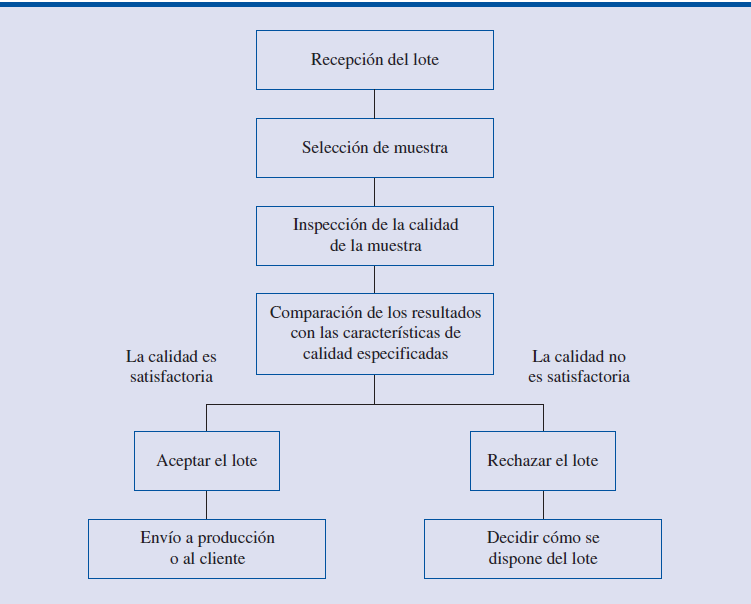
\includegraphics[width=9.5cm]{IMAGENES/MA.png}
        \label{figura1}
\end{figure}
\end{frame}

\begin{frame}
\frametitle{Marco Teórico}
~\\El muestreo de aceptación puede dividirse en dos tipos fundamentales dependiendo de la característica observada:
\begin{itemize}
\item Muestreo por atributos: cuando en la inspección los artículos se dividen en defectuosos y en no defectuosos, según cumplan con un conjunto de requerimientos.
\item Muestreo por variables: cuando en la inspección se mide una variable cuantitativa: longitudes, pesos... y se evalúa la distancia entre dicha cantidad y la requerida en las especificaciones.
\end{itemize}
\end{frame}

\begin{frame}
\frametitle{Marco Teórico}

\end{frame}

\begin{frame}
\frametitle{Marco Teórico}

\end{frame}
\end{document}